\documentclass{article}
\usepackage[utf8]{inputenc}
\usepackage{amsmath}
\usepackage{mathtools}
\usepackage{float}
\usepackage[numbered, framed]{matlab-prettifier}
\usepackage[font=small]{caption}


\setlength{\abovecaptionskip}{3pt}
\setlength{\belowcaptionskip}{3pt}

\title{Control Theory Homework 2}
\author{Kamil Kamaliev (k.kamaliev@innopolis.university), Var e}
\date{March 2020}

\begin{document}
    \maketitle
    
    \paragraph{2.}
    
        \leavevmode
        \textbf{Calculating Total TF.}
        
         \begin{figure}[hbt!]
            \centering
            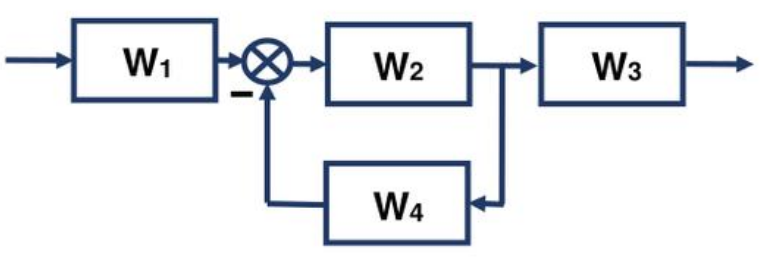
\includegraphics[scale=0.3]{hm2_2.png}
            \caption{Closed Loop System with 2 inputs.}
        \end{figure}
        
         \vskip
        We can see that $W_2$ and $W_4$ are in feedback loop.
        
        Thus we can combine them $W_{24} = \frac{W_2}{1 + W_2 * W_4}$
        
        \bigbreak
        Next, notice that $W_1, \ W_{24} \ and \ W_3$ are in series connection.
        
        Thus we can combine them into Total TF $W_0 = W_1 * \frac{W_2}{1 + W_2 * W_4} * W_3$
        
        \bigbreak
        After substituting corresponding values of $W_1, \ W_2, \ W_3 \ and \ W_4$, we obtain:
        
        $$W_0 = \frac{2}{s+1} * \frac{1}{s} * \frac{1}{1 + \frac{1}{s} * \frac{1}{s+3}} * \frac{2}{s+1.5} = \frac{4s + 12}{s^4 + 5.5s^3 + 10s^2 + 7s + 1.5}$$
        
        \noindent
        \textbf{Schemas}
        
        \begin{figure}[hbt!]
            \centering
            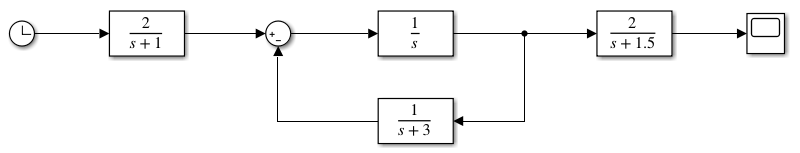
\includegraphics[scale=0.4]{ct_hm2_2_shortTF.png}
            \caption{Original Schema.}
        \end{figure}
        
        \begin{figure}[hbt!]
            \centering
            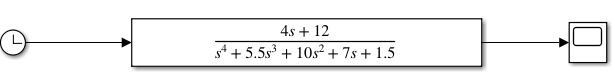
\includegraphics[scale=0.5]{ct_hm2_2_usualTFs.png}
            \caption{Simplified Schema.}
        \end{figure}
        
        
        \newpage
        
        \noindent
        \textbf{Plots}
        
        \smallbreak
        There are only 2 lines because original and total TFs coincide.
        
        \begin{figure}[hbt!]
            \centering
            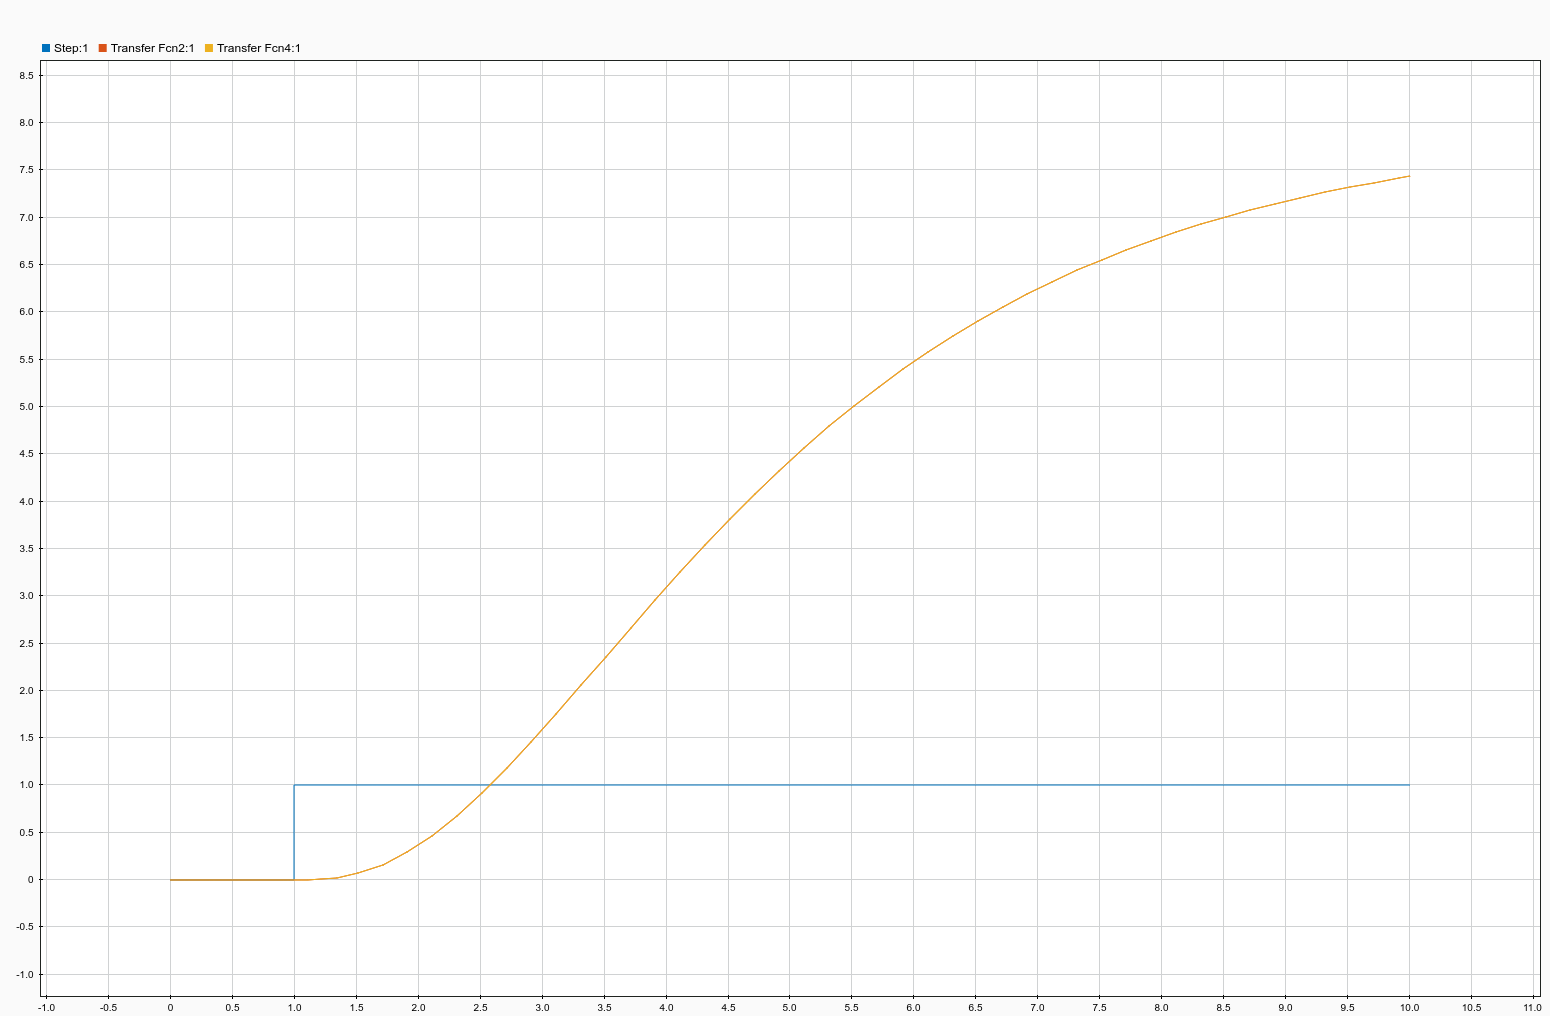
\includegraphics[scale=0.3]{hm2_stepplot.png}
            \caption{Step Plot.}
        \end{figure}
        
        \begin{figure}[hbt!]
            \centering
            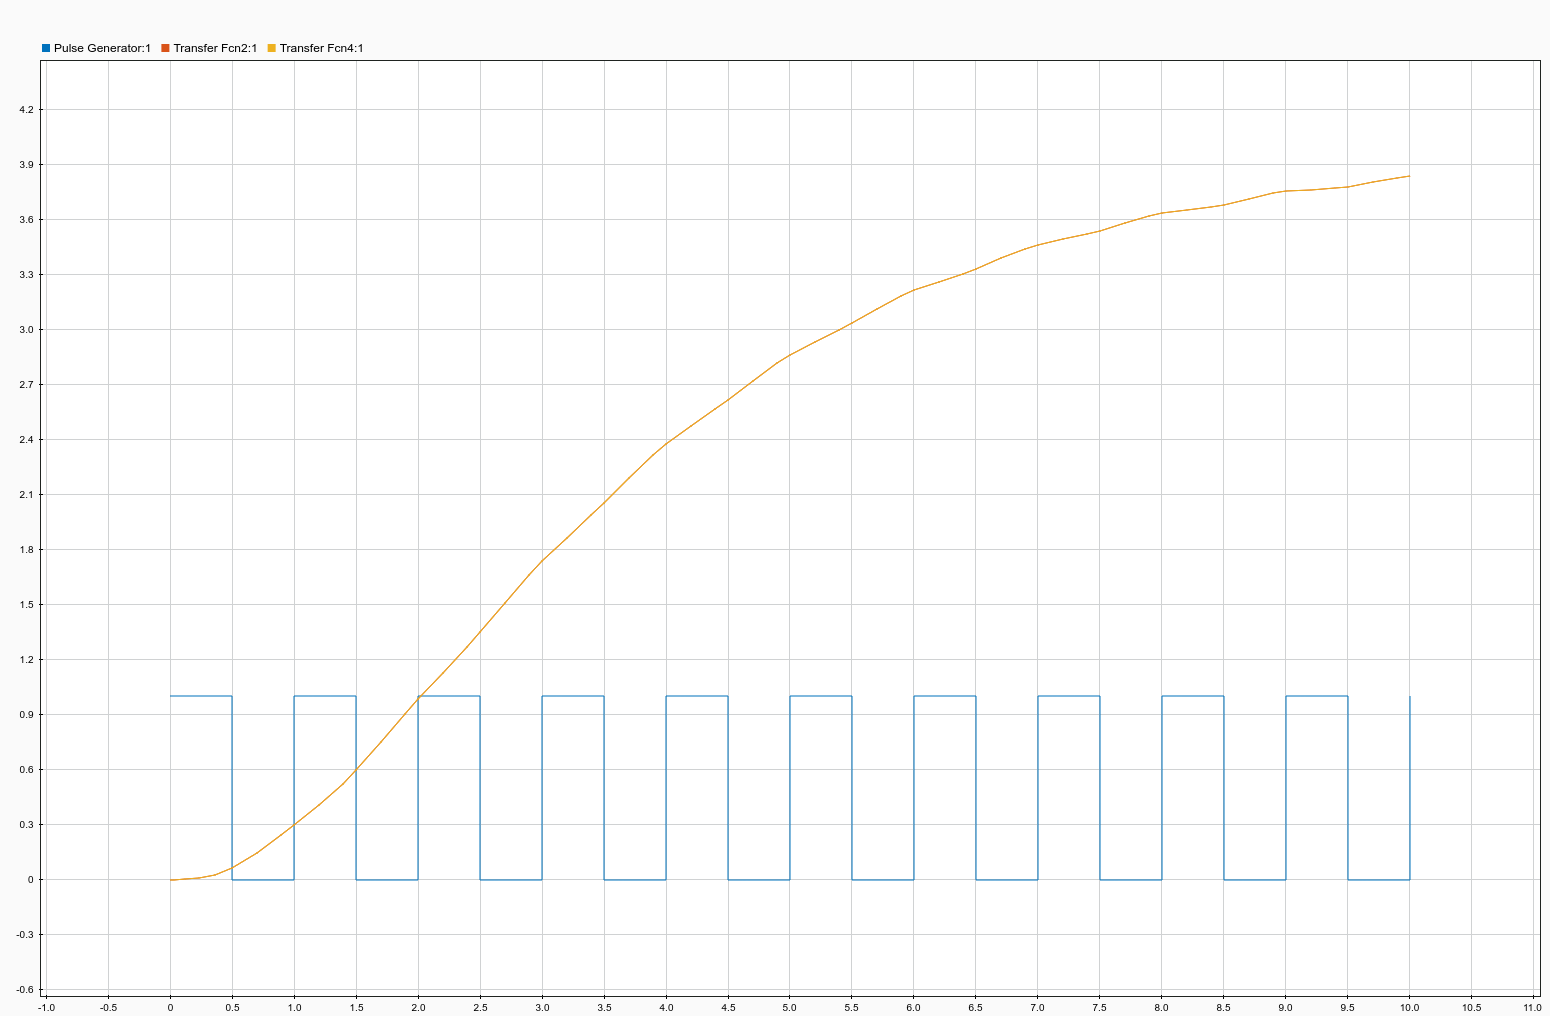
\includegraphics[scale=0.3]{hm2_impulseplot.png}
            \caption{Impulse Plot (Period T = 1, Pulse Width is 50\%).}
        \end{figure}
    
        \begin{figure}[hbt!]
            \centering
            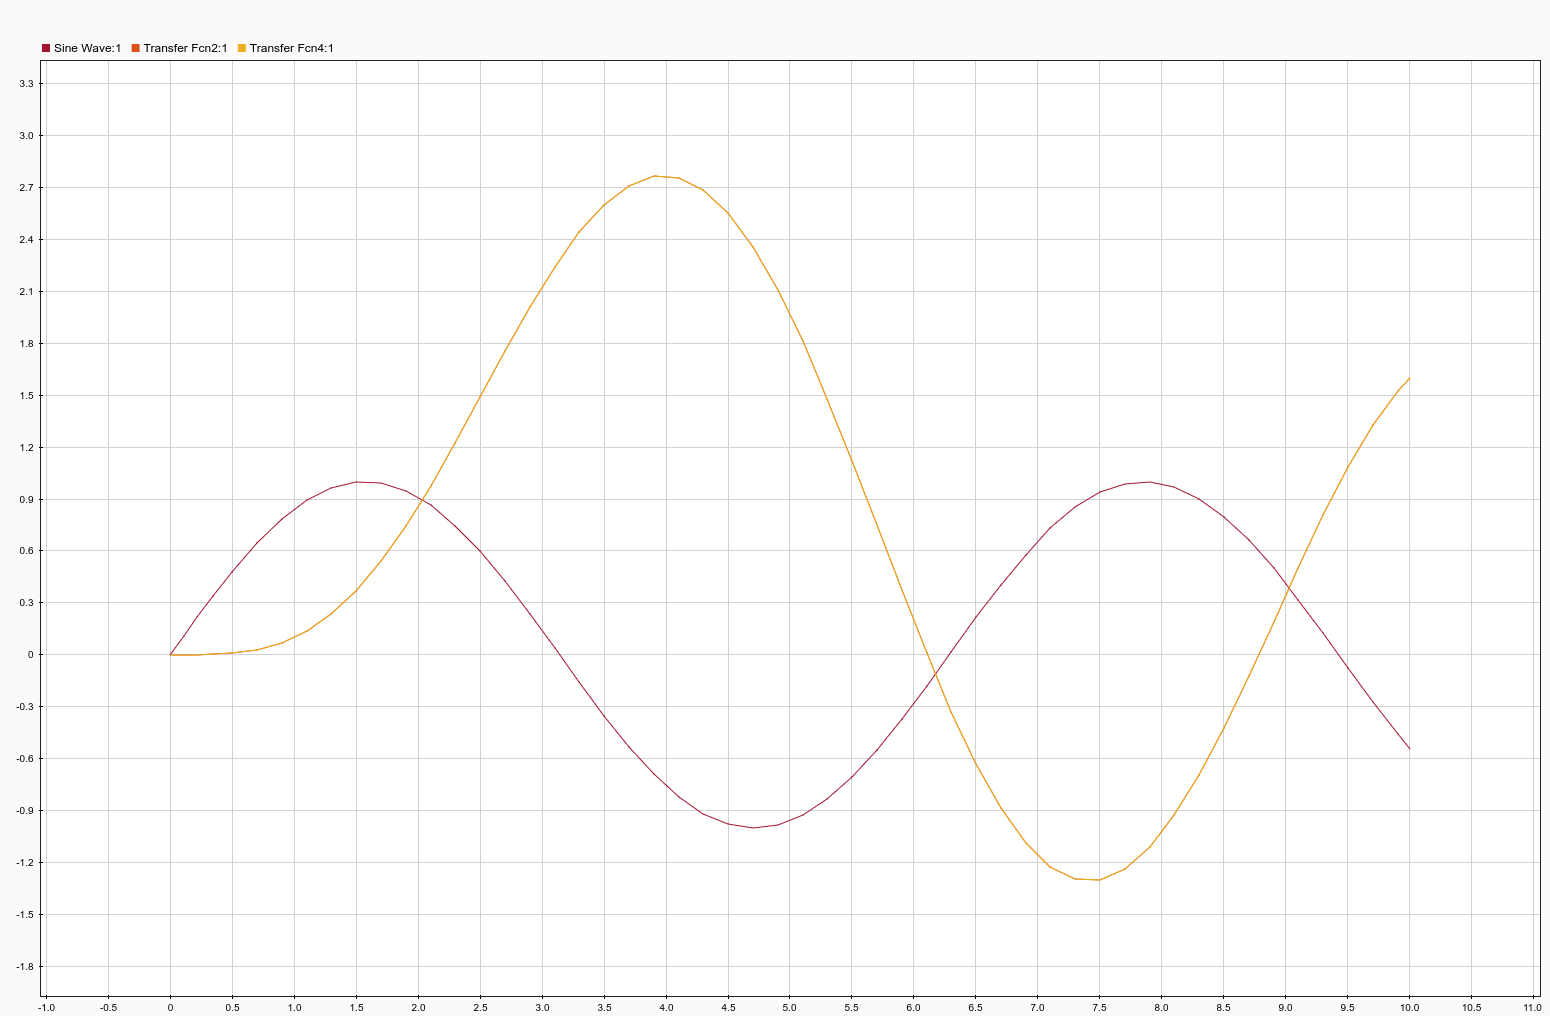
\includegraphics[scale=0.3]{hm2_frequencyplot.png}
            \caption{Frequency Plot (Sine is used without any shift or scale).}
        \end{figure}
        
        \newpage
        
        \noindent
        \textbf{Bode and Pole-Zero plots.}
        
        Sine is used (no scale or shift).
        
        \begin{figure}[hbt!]
            \centering
            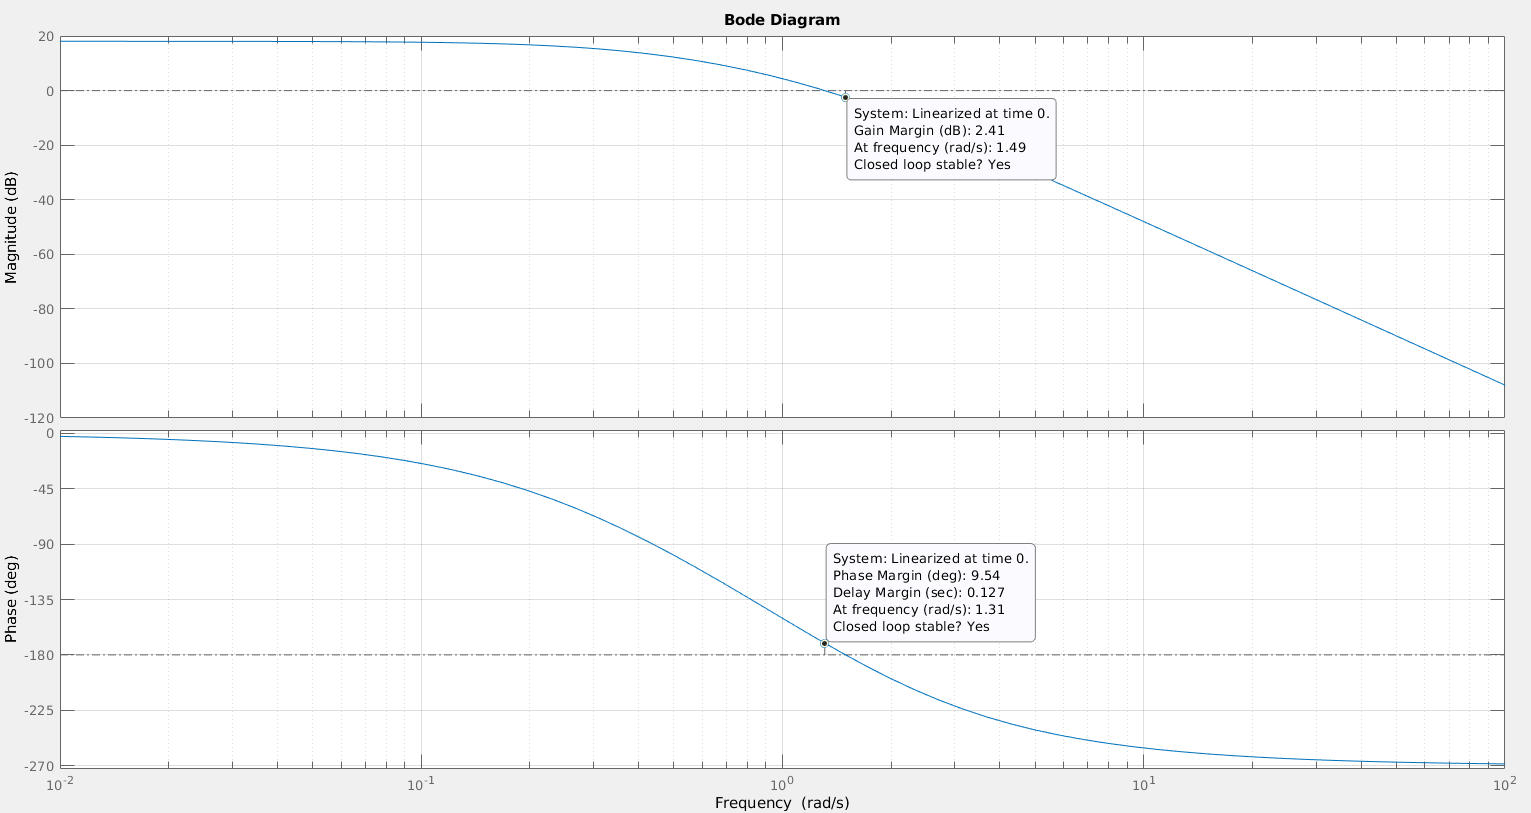
\includegraphics[scale=0.2]{hm2_bodeplot.png}
            \caption{Bode Plot.}
        \end{figure}
    
        \begin{figure}[hbt!]
            \centering
            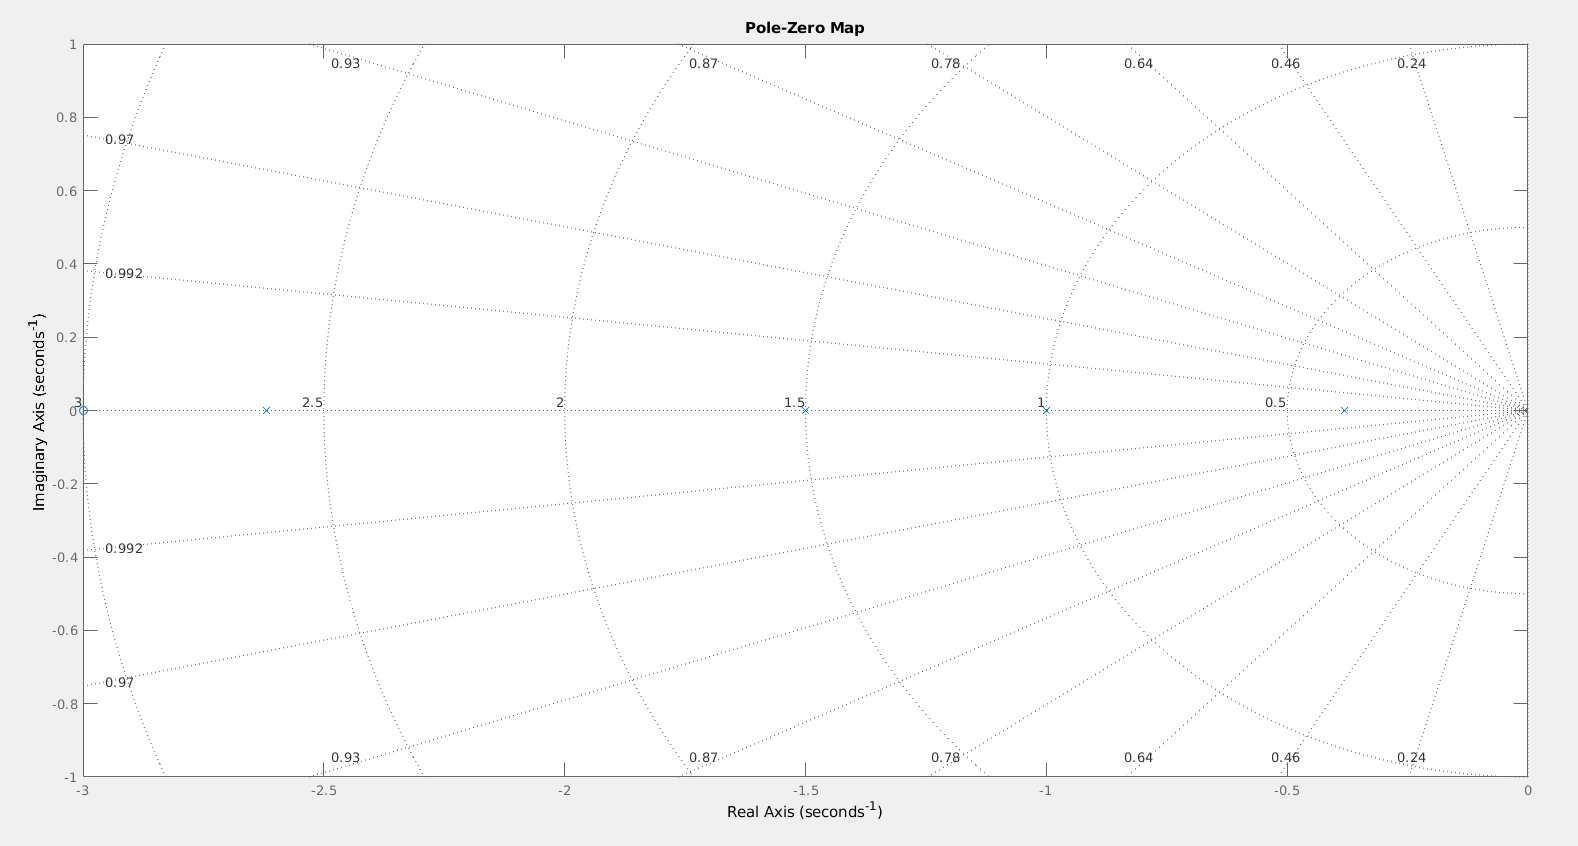
\includegraphics[scale=0.2]{hm2_polezeroplot.png}
            \caption{Pole-Zero Plot.}
        \end{figure}
        
        
        As you can see from pictures, the system is stable (all points in Pole-Zero are in negative real axis).
        
        \bigbreak
    
        
        \textbf{Bode plot analysis.}
            \smallbreak
        Let's rewrite our TF:
        
         $$W_0 = \frac{4s + 12}{s^4 + 5.5s^3 + 10s^2 + 7s + 1.5} = \frac{4(s+3)}{(s + 0.381966)(s+1)(s+1.5)(s+2.61803)}$$
        
        Zero: -3
        
        Poles: -0.381966, -1, -1.5, -2.61803
        
        As you can see on Figure 7, Margin plot intersects zero at 1.49 and Phase plot intersects -180 at 1.31.
        
        
        \newpage
        
        \paragraph{3.}
        
        \smallbreak
        
        We have the following schema:
        
        \begin{figure}[hbt!]
            \centering
            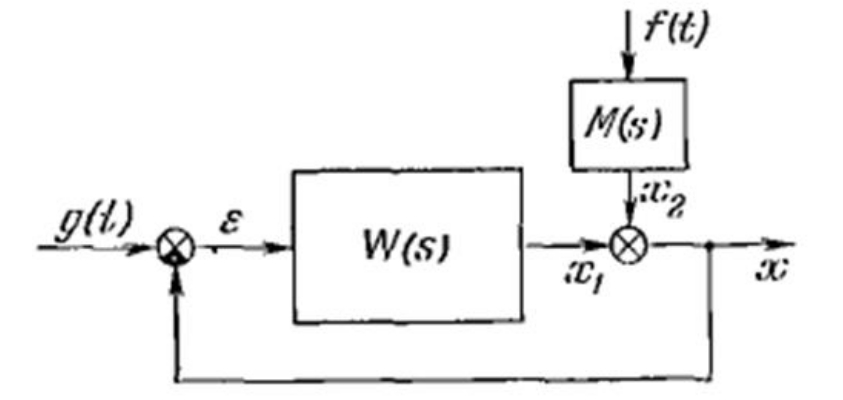
\includegraphics[scale=0.2]{hm2_schema.png}
            \caption{Closed Loop System with 2 inputs.}
        \end{figure}
        
        In system with 2 inputs, to calculate total TF $W_0$, we need to calculate TFs for each input individually (omitting other input).
        
        \bigbreak
        
        Let's find TF with respect to $g(t)$ first.
        
        After "hiding" $f(t)$, we are left with negative feedback loop. Hence,
        
        $$\frac{X}{G} = \frac{W(s)}{1 + W(s)}$$
        
        Now, let's perform the similar actions with respect to $g(t)$.
        
        After "hiding" $g(t)$, we are left with the following schema:
        
        \begin{figure}[hbt!]
            \centering
            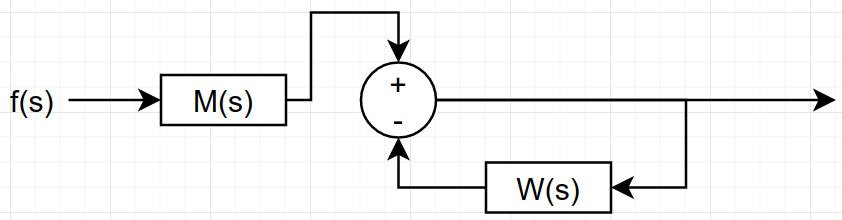
\includegraphics[scale=0.2]{hm2_3.png}
            \caption{Schema when omitting g(t).}
        \end{figure}
        
        Which is a serial connection of $M(s)$ and a feedback loop.
        Thus we can reduce it to 
        
        $$\frac{X}{F} = \frac{M(s)}{1 + W(s)}$$
        
        
        After substituting corresponding values of $M(s) \ and \ W(s)$ we obtain:
        
        $$\frac{X}{G} = \frac{s-1}{s^2 - s + 1} * \frac{1}{ 1 + \frac{s-1}{s^2 - s + 1}} = \frac{s-1}{s^2}$$
        
        $$\frac{X}{F} = \frac{s+1}{s + 3} * \frac{1}{ 1 + \frac{s-1}{s^2 - s + 1}} = \frac{s^3 + 1}{s^3 + 3s^2}$$
        
        $$X = \frac{X}{G} \cdot G + \frac{X}{F} \cdot F = \frac{s-1}{s^2} \cdot G + \frac{s^3 + 1}{s^3 + 3s^2} \cdot F$$
            
        \paragraph{4.}
        
        At first, let's derive a formula allowing us to find TF of SS.
        
        $$\left\{ \begin{array}{ll} 
                x^\prime = Ax + Bu\\
                y = Cx + Du
            \end{array} \right.$$
        
        $$\left\{ \begin{array}{ll} 
                sX = AX + BU\\
                Y = CX + DU
            \end{array} \right.$$
        $$(sI-A)X = BU$$
        $$X = (sI-A)^{-1}BU$$
        
        And now let's substitute X into Y's equation.
        $$Y = C(sI-A)^{-1}BU + DU$$
        Hence, our TF $W_0$ is:
        $$W_0 = C(sI-A)^{-1}B + D$$
 
        Now, let's substitute corresponding values from variant e into the equation.
        
        $$W_0 = 
            \begin{bmatrix}
                0 & 1
            \end{bmatrix} (s \cdot
            \begin{bmatrix}
                1 & 0\\
                0 & 1
            \end{bmatrix} - 
            \begin{bmatrix}
                -1 & 2\\
                0 & 1
            \end{bmatrix})^{-1}
            \begin{bmatrix}
                1\\
                1
            \end{bmatrix} + 
            \begin{bmatrix}
                3
            \end{bmatrix}$$
       
        $$W_0 = 
            \begin{bmatrix}
                0 & 1
            \end{bmatrix}
            \begin{bmatrix}
                s+1 & -2\\
                0 & s-1
            \end{bmatrix}^{-1}
            \begin{bmatrix}
                1\\
                1
            \end{bmatrix} + 
            \begin{bmatrix}
                3
            \end{bmatrix}$$
            
            
        $$W_0 = 
            \begin{bmatrix}
                0 & 1
            \end{bmatrix}
            \begin{bmatrix}
                \frac{1}{s-1}\\
                \frac{1}{s-1}
            \end{bmatrix} + 
            \begin{bmatrix}
                3
            \end{bmatrix}$$
            
        $$W_0 = \frac{1}{s-1} + 3$$
        
        $$W_0 = \frac{3s - 2}{s-1}$$
        
        
    
    
    \paragraph{5.}
        Use the formula for TF derived in previous exercise:
        $$W_0 = C(sI-A)^{-1}B + D$$
 
        Substitute corresponding values from variant e into the equation.
        
        $$W_0 = 
            \begin{bmatrix}
                3 & 0
            \end{bmatrix} (s \cdot
            \begin{bmatrix}
                1 & 0\\
                0 & 1
            \end{bmatrix} - 
            \begin{bmatrix}
                1 & -2\\
                1 & 1
            \end{bmatrix})^{-1}
            \begin{bmatrix}
                1 & 2\\
                2 & 1
            \end{bmatrix} + 
            \begin{bmatrix}
                0 & 3
            \end{bmatrix}$$
       
        $$W_0 = 
            \begin{bmatrix}
                3 & 0
            \end{bmatrix}
            \begin{bmatrix}
                s - 1 & 2\\
                -1 & s - 1
            \end{bmatrix}^{-1}
            \begin{bmatrix}
                1 & 2\\
                2 & 1
            \end{bmatrix} + 
            \begin{bmatrix}
                0 & 3
            \end{bmatrix}$$
            
            
        $$W_0 = 
            \frac{1}{s^2 - 2s + 3}
            \begin{bmatrix}
                3 & 0
            \end{bmatrix}
             \begin{bmatrix}
                s - 1 & -2\\
                1 & s - 1
            \end{bmatrix}
             \begin{bmatrix}
                1 & 2\\
                2 & 1
            \end{bmatrix} + 
            \begin{bmatrix}
                0 & 3
            \end{bmatrix}$$
            
         $$W_0 = \frac{3}{s^2 - 2s + 3}
            \begin{bmatrix}
                s-5 & 2s-4
            \end{bmatrix}$$
            
        $$W_0 =
        \begin{bmatrix}
                \frac{3s-15}{s^2-2s+3} & \frac{3s^2-3}{s^2-2s+3}
        \end{bmatrix}$$
        
        We got a matrix. Hence, the system has 2 inputs.
   
        
    \paragraph{6.}
        
        Notice that we have to inputs f and x.
        
        
        \begin{figure}[hbt!]
            \centering
            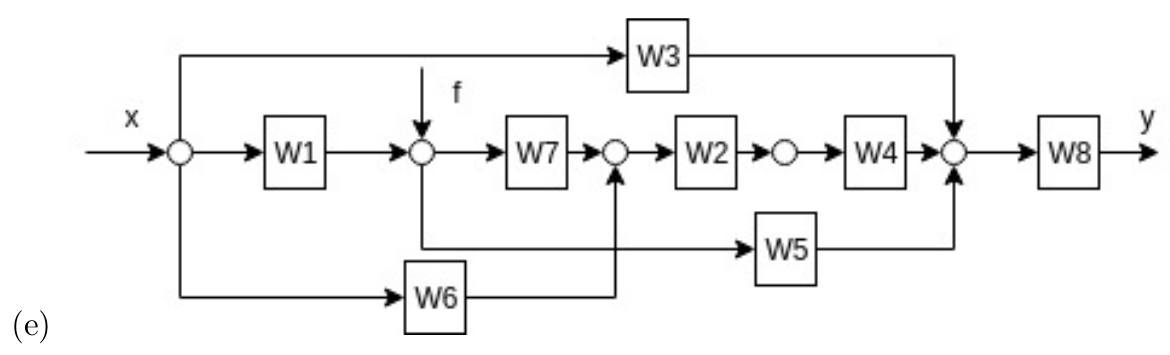
\includegraphics[scale=0.2]{hm2_6_1.png}
            \caption{Given Schema.}
        \end{figure}
        
        First, let's set x to 0 and calculate TF for f: 
        
         \begin{figure}[hbt!]
            \centering
            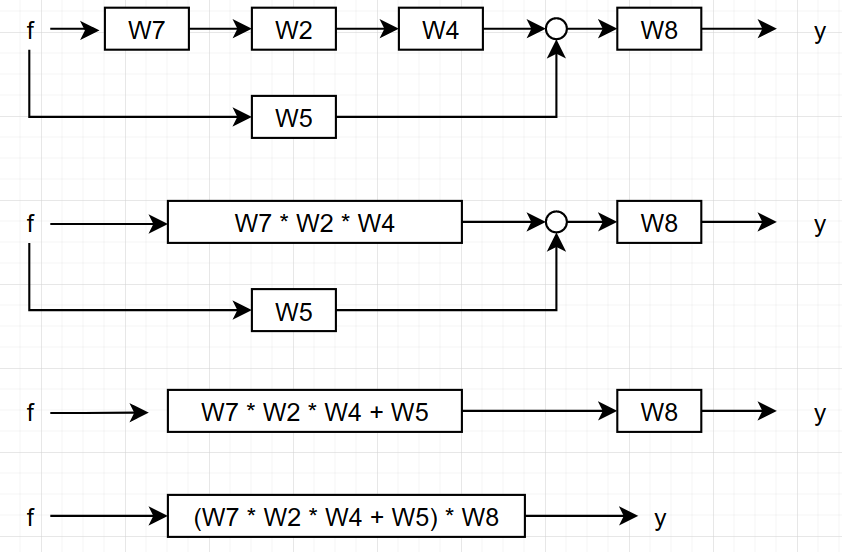
\includegraphics[scale=0.3]{hm2_6f.png}
            \caption{Finding TF for f.}
        \end{figure}
        
        Hence, $\frac{Y}{F} = (W_7 \cdot W_2 \cdot W_4 + W_5) \cdot W_8$
        
        \bigbreak
        
        Now, set f to 0 and calculate TF for x.
        
        (Latex doesn't want to put picture here, so, please, scroll down to see steps for finding TF for x).
        \bigbreak
        
        Hence, $\frac{Y}{X} = (W_1 \cdot W_5 + W_3 + W_2 \cdot W_4 \cdot (W_1 \cdot W_7 + W_6)) \cdot W_8$
        
        As a result, we have 
        $$\frac{Y}{F} \cdot F + \frac{Y}{X} \cdot X $$
        
        where
        
        $$\frac{Y}{X} = (W_1 \cdot W_5 + W_3 + W_2 \cdot W_4 \cdot (W_1 \cdot W_7 + W_6)) \cdot W_8$$
        
        and
        
        $$\frac{Y}{F} = (W_7 \cdot W_2 \cdot W_4 + W_5) \cdot W_8$$
        
         \begin{figure}[hbt!]
            \centering
            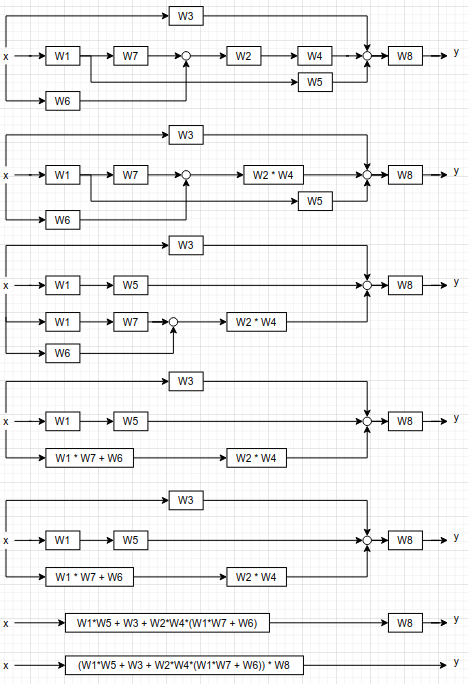
\includegraphics[scale=0.7]{hm_6x3.png}
            \caption{Finding TF for x.}
        \end{figure}
        
        
\end{document}